\subsection{Anschluss}

\begin{figure}[ht]
  \centering
  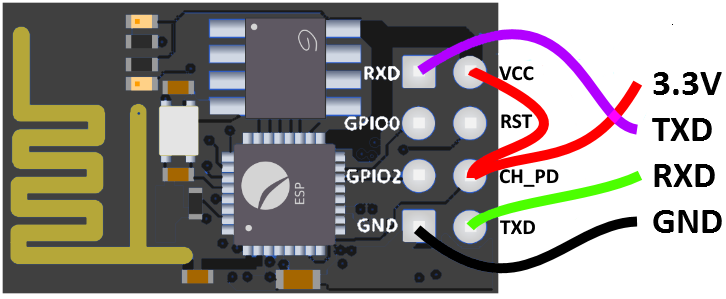
\includegraphics[scale=0.42]{images/ESP8266.png}	
  %	\caption{}
  \label{ESP8266-01}
\end{figure}


\begin{figure}[ht]
  \centering
  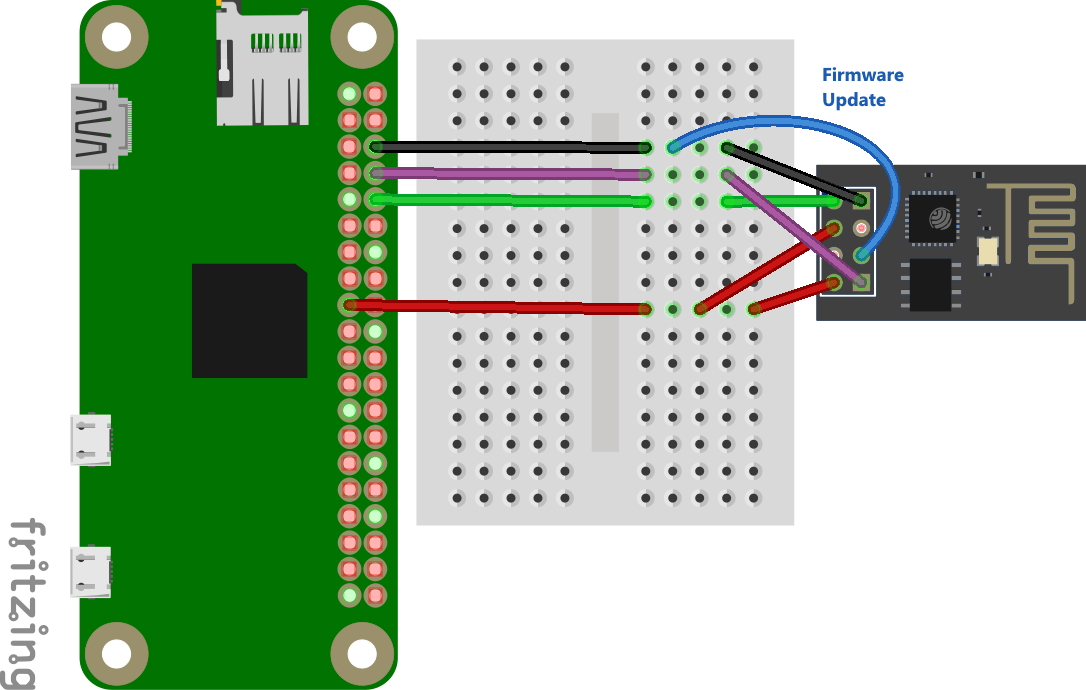
\includegraphics[scale=1.00]{images/ESP8266_ESP-01.png}	
  %	\caption{}
  \label{ESP8266_ESP-01}
\end{figure}

\subsection{Firmware Update}

%Quelle: https://www.allaboutcircuits.com/projects/flashing-the-ESP-01-firmware-to-SDK-v2.0.0-is-easier-now/
Tools: \url{http://www.espressif.com/en/support/download/other-tools}\\
SDKs und Demos: \url{http://www.espressif.com/en/support/download/sdks-demos}\\
NONOS SDK Source: \url{https://github.com/espressif/ESP8266_NONOS_SDK/releases}\\
Download NONOS SDK: \url{https://github.com/espressif/ESP8266_NONOS_SDK/archive/v2.1.0.zip}\\

Um das Firmware Update ausf�hren zu k�nnen muss der GPIO0 Eingang auf GND gesetzt werden. Das kann entweder dauerhaft gemacht werden indem der Pin direkt auf GND verbunden wird. Oder man macht es �ber einen Schalter. Dann ist wichtig, dass der Schalter w�hrend des Boot-Vorgangs bzw. bevor Reset gedr�ckt wird, gedr�ckt gehalten wird. Ich w�rde aber empfehlen einfach den GPIO0 Pin �ber eine Kabel auf GND zu verbinden. Reset kann ausgel�st werden durch entfernen und zur�ckstecken der 3,3~V Versorgung.

Beim ESP-01 (8~MBit) m�ssen folgende Dateien und Adressen �bertragen werden.    

\begin{table}[h]
\caption{ESP01 (8~MBit) Firmware Dateien}
\centering
\begin{tabular}{|l|c|c|}
\hline
\textbf{Datei (NONOS SDK)} & \textbf{Adresse} \\
\hline
\path{bin/blank.bin} & 0xFB000\\
\hline
\path{bin/esp_init_data_default.bin} & 0xFC000\\
\hline
\path{bin/blank.bin} & 0x7E000\\
\hline
\path{bin/blank.bin} & 0xFE000\\
\hline
\path{bin/boot_v1.6.bin} & 0x00000\\
\hline
\path{bin/at/512+512/user1.1024.new.2.bin} & 0x01000\\
\hline
\end{tabular}
\end{table}



\subsubsection{Linux (Raspberry Pi)}

\begin{console}
cd ~
wget https://github.com/espressif/ESP8266_NONOS_SDK/archive/v2.1.0.zip
unzip v2.1.0.zip
sudo apt-get install python python-pip
sudo pip install esptool
\end{console}

%pip2 install esptool


\begin{console}
esptool.py version
\end{console}

\begin{screensmall}
esptool.py v2.1
2.1
\end{screensmall}

\begin{console}
python esptool.py -p /dev/ttyAMA0 flash_id 
\end{console}


%ttyUSB0 
\begin{console}
cd ESP8266_NONOS_SDK-2.1.0/bin/
sudo esptool.py -p /dev/ttyAMA0 write_flash 0x00000 boot_v1.6.bin 0x01000 at/512+512/user1.1024.new.2.bin \
 0xFB000 blank.bin 0xFC000 esp_init_data_default.bin 0x7E000 blank.bin 0xFE000 blank.bin 
\end{console}



%
\subsubsection{Windows}


Download Flash Tool: \url{http://www.espressif.com/sites/default/files/tools/flash_download_tools_v3.4.9.2_0.zip}\\

Nach dem Download des letzten Release des NONOS SDK und des Flash Tool m�ssen beide Archive entpackt werden.
Dann kann das Flash Tool "`ESPFlashDownloadTool\_v3.4.9.2.exe"' gestartet werden. Nun  muss die korrekte COM-Nummer ausgew�hlt und die Bautrate auf 115200 gestellt werden. Danach kann mit der Start Taste der ESP gesucht werden. Wenn dies erfolgreich ist werden verschiedene Daten der Platine ausgelesen und im Fenster angezeigt.\\
Dann k�nnen die verschienden Dateien der neuen Firmware aus dem "`bin"' Verzeichnis des NONOS SDKs ausgew�hlt werden. Zu jeder Datei muss noch eine Start-Adresse eingeben werden.\\
Beim ESP-01 (8~MBit) m�ssen die angegebenen Dateien und Adressen eingegeben und �bertragen werden.    

\begin{figure}[ht]
  \centering
  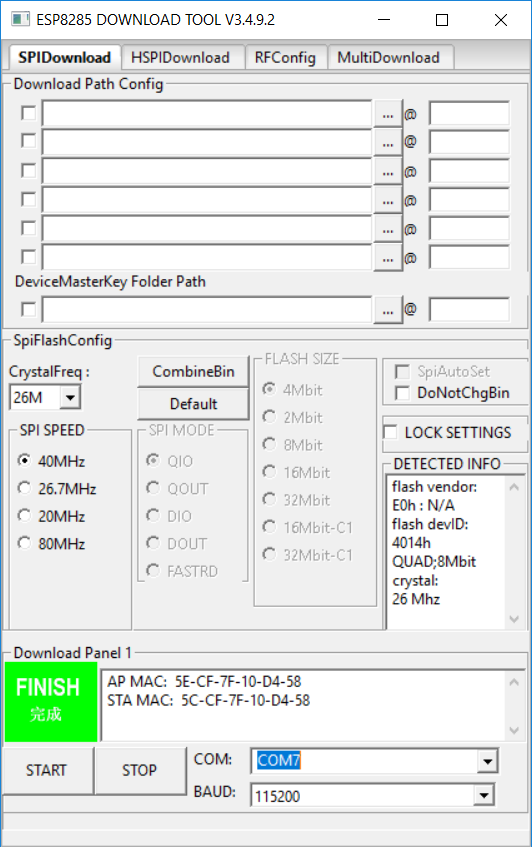
\includegraphics[scale=1.00]{images/ESP8266-ESP_01_FW_update_1.png}	
  %	\caption{}
  \label{ESP8266_ESP-01_FW_UPDATE_1}
\end{figure}

Danach kann mit der Start Taste die Aktualisierung gestartet werden. Wenn der blaue Balken das Ende erreicht hat, kann der ESP aus- und wieder angesteckt werden. Nun sollte die neue Firmware aktiv sein. Mit einem Terminalprogramm wie Putty (COM Verbindung) kann die Version abgefragt werden.

\begin{figure}[ht]
  \centering
  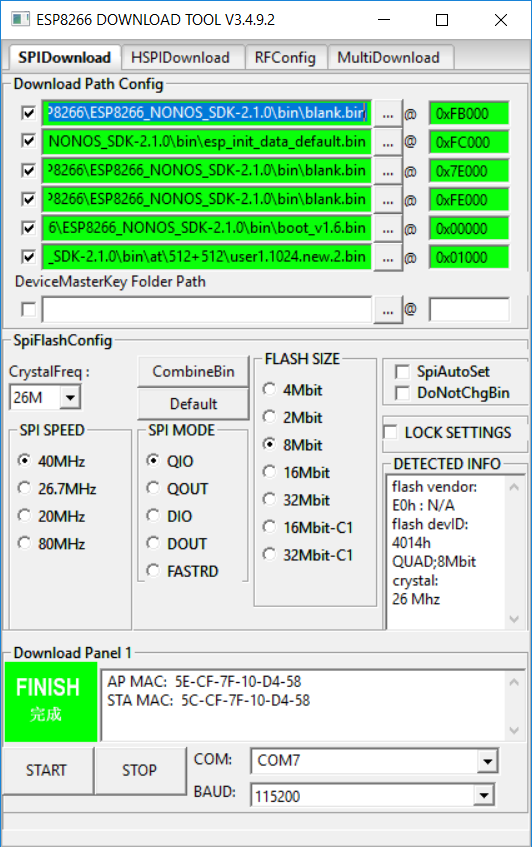
\includegraphics[scale=1.00]{images/ESP8266-ESP_01_FW_update_2.png}	
  %	\caption{}
  \label{ESP8266_ESP-01_FW_UPDATE_2}
\end{figure}


\begin{figure}[ht]
  \centering
  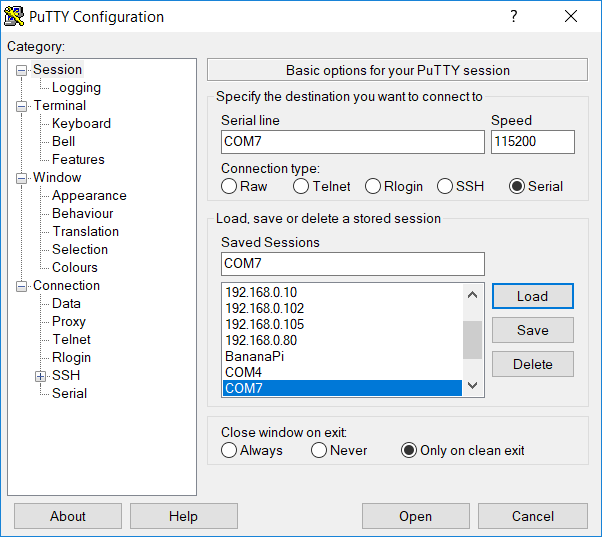
\includegraphics[scale=1.00]{images/Putty_COM.png}	
  %	\caption{}
  \label{Putty_COM}
\end{figure}

\begin{console}
Version abfragen: AT+GMR
\end{console}
\framebox{Enter} \framebox{Strg}+\framebox{J} 


\begin{screensmall}
AT version:1.4.0.0(May  5 2017 16:10:59)
SDK version:2.1.0(116b762)
compile time:May  5 2017 16:37:48
OK
\end{screensmall}



\subsection{Verwendung}


\textbf{AT-Befehlsatz:}\\
\url{https://www.itead.cc/wiki/images/5/53/Esp8266_at_instruction_set_en_v1.5.4_0.pdf}\\

\begin{figure}[ht]
  \centering
  
\includegraphics[scale=0.2]{images/QR_ESP8266_AT-Cmd.png}	
  %	\caption{}
  \label{ESP8266_AT-Cmd}
\end{figure}


\textbf{Raspberry Pi:}
\begin{console}
sudo systemctl stop serial-getty@ttyAMA0.service
sudo systemctl status serial-getty@ttyAMA0.service
sudo apt-get install minicom
sudo minicom -b 115200 -o -D /dev/ttyAMA0
\end{console}

\textbf{USB UART:} 
\begin{console}
sudo apt-get install minicom
sudo minicom -b 115200 -o -D /dev/ttyUSB0
\end{console}

\textbf{Beispielkommunikation:}

Verbindungstest:
\begin{console}
 AT
\end{console}
\framebox{Enter} \framebox{Strg}+\framebox{J} 

\begin{screensmall}
OK
\end{screensmall}

Reset:
\begin{console}
 AT+RST
\end{console}
\framebox{Enter} \framebox{Strg}+\framebox{J}
\begin{screensmall}
 ets Jan  8 2013,rst cause:2, boot mode:(3,6)

load 0x40100000, len 1396, room 16
tail 4
chksum 0x89
load 0x3ffe8000, len 776, room 4
tail 4
chksum 0xe8
load 0x3ffe8308, len 540, room 4
tail 8
chksum 0xc0
csum 0xc0

2nd boot version : 1.4(b1)
  SPI Speed      : 40MHz
  SPI Mode       : DIO
  SPI Flash Size & Map: 8Mbit(512KB+512KB)
jump to run user1 @ 1000

Ai-Thinker Technology Co.,Ltd.

ready
\end{screensmall}

Version abfragen:
\begin{console}
AT+GMR
\end{console}
\framebox{Enter} \framebox{Strg}+\framebox{J}

\begin{screensmall}
AT version:0.40.0.0(Aug  8 2015 14:45:58)
SDK version:1.3.0
Ai-Thinker Technology Co.,Ltd.
Build:1.3.0.2 Sep 11 2015 11:48:04
OK
\end{screensmall}

WLAN Modus Station setzen:
\begin{console}
 AT+CWMODE=1
\end{console}
\framebox{Enter} \framebox{Strg}+\framebox{J}


\begin{screensmall}
OK
\end{screensmall}

Gefundene WLAN-Netze auflisten:
\begin{console}
 AT+CWLAP
\end{console}
\framebox{Enter} \framebox{Strg}+\framebox{J}


\begin{screensmall}
+CWLAP:(3,"NETGEAR86",-86,"a0:63:91:ca:98:ca",6,-14)
+CWLAP:(4,"A1-PMC",-78,"a4:b1:e9:43:f4:d3",11,-41)
+CWLAP:(4,"Home",-92,"f4:06:8d:3b:e1:3c",11,-41)
+CWLAP:(3,"AndroidAP",-89,"10:a5:d0:73:de:eb",11,23)
\end{screensmall}

Minicom beenden:\\
\framebox{Strg} \framebox{A} \framebox{X}

